\subsubsection{Internal modifications}
\label{sec:internal_modifications}
\begin{figure}[!htbp]
\centering
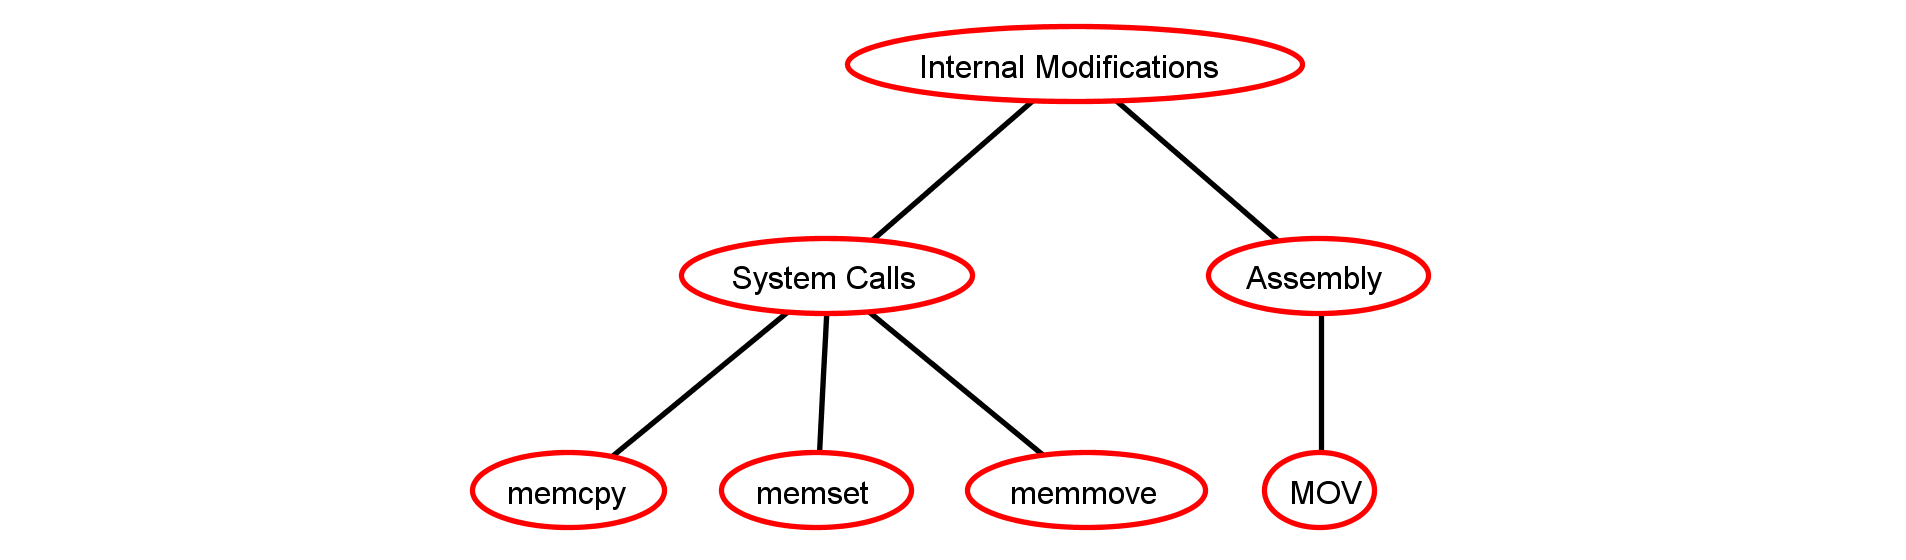
\includegraphics[width=\textwidth, keepaspectratio]{sections/adtrees/InternalModificationsWithoutDefenses.png}
\caption{This attack tree shows possible attacks that are grouped under internal modification}
\label{fig:attacks_internal}
\end{figure}
A group of attack is internal modifications which is in contrast to external modifications occurring from inside the process virtual memory. As the attacker is already inside the virtual memory, modification is easier and less restricted than the previously shown external modifications. The attacker can make use of existing functions like \syscall{memcpy} or \syscall{memset}, to modify the values inside memory, without having to use the indirection via \syscall{WriteProcessMemory}. Besides the present \syscall{mem*} functions, the attacker can also make use of assembly code. Figure \ref{fig:attacks_internal} shows this type of attack in node [2.1]. The assembly node [2.2] shows an alternative way to achieve the same result  as [2.1]. With assembly, instruction are executed and the indirection of using function calls is removed.  

\medskip

The shown attacks are combined in Figure \ref{fig:attacks}, containing now both parts of attacks, external and internal modifications.